%%%%%%%%%%%%%%%%%%%%%%%%%%%%%%%%%%%%%%%%%%%%%%%%%%%%%%%%%%%%%%%%%%%%%%%%%%%%
% AGUJournalTemplate.tex: this template file is for articles formatted with LaTeX
%
% This file includes commands and instructions
% given in the order necessary to produce a final output that will
% satisfy AGU requirements, including customized APA reference formatting.
%
% You may copy this file and give it your
% article name, and enter your text.
%
%
% Step 1: Set the \documentclass
%
%

%% To submit your paper:
\documentclass[draft]{agujournal2019}
\usepackage{url} %this package should fix any errors with URLs in refs.
\usepackage{lineno}
\usepackage[inline]{trackchanges} %for better track changes. finalnew option will compile document with changes incorporated.
\usepackage{soul}
\usepackage{ragged2e}
\justifying
%\linenumbers

%%%%%%%
% As of 2018 we recommend use of the TrackChanges package to mark revisions.
% The trackchanges package adds five new LaTeX commands:
%
%  \note[editor]{The note}
%  \annote[editor]{Text to annotate}{The note}
%  \add[editor]{Text to add}
%  \remove[editor]{Text to remove}
%  \change[editor]{Text to remove}{Text to add}
%
% complete documentation is here: http://trackchanges.sourceforge.net/
%%%%%%%

\draftfalse

%% Enter journal name below.
%% Choose from this list of Journals:
%
% JGR: Atmospheres
% JGR: Biogeosciences
% JGR: Earth Surface
% JGR: Oceans
% JGR: Planets
% JGR: Solid Earth
% JGR: Space Physics
% Global Biogeochemical Cycles
% Geophysical Research Letters
% Paleoceanography and Paleoclimatology
% Radio Science
% Reviews of Geophysics
% Tectonics
% Space Weather
% Water Resources Research
% Geochemistry, Geophysics, Geosystems
% Journal of Advances in Modeling Earth Systems (JAMES)
% Earth's Future
% Earth and Space Science
% Geohealth
%
% ie, \journalname{Water Resources Research}

\journalname{Water Resources Research}


\begin{document}

%% ------------------------------------------------------------------------ %%
%  Title
%
% (A title should be specific, informative, and brief. Use
% abbreviations only if they are defined in the abstract. Titles that
% start with general keywords then specific terms are optimized in
% searches)
%
%% ------------------------------------------------------------------------ %%

% Example: \title{This is a test title}

\title{Predicción de caudales medios diarios por medio de modelos de inteligencia artificial y aprendizaje automático}

%% ------------------------------------------------------------------------ %%
%
%  AUTHORS AND AFFILIATIONS
%
%% ------------------------------------------------------------------------ %%

% Authors are individuals who have significantly contributed to the
% research and preparation of the article. Group authors are allowed, if
% each author in the group is separately identified in an appendix.)

% List authors by first name or initial followed by last name and
% separated by commas. Use \affil{} to number affiliations, and
% \thanks{} for author notes.
% Additional author notes should be indicated with \thanks{} (for
% example, for current addresses).

% Example: \authors{A. B. Author\affil{1}\thanks{Current address, Antartica}, B. C. Author\affil{2,3}, and D. E.
% Author\affil{3,4}\thanks{Also funded by Monsanto.}}

\authors{Juan Esteban Taborda Soto\affil{1}\thanks{ORCID: https://orcid.org/0000-0002-1908-6030}}

\affiliation{1}{Universidad Nacional de Colombia}
% \affiliation{2}{Second Affiliation}
% \affiliation{3}{Third Affiliation}
% \affiliation{4}{Fourth Affiliation}

%(repeat as many times as is necessary)

%% Corresponding Author:
% Corresponding author mailing address and e-mail address:

% (include name and email addresses of the corresponding author.  More
% than one corresponding author is allowed in this LaTeX file and for
% publication; but only one corresponding author is allowed in our
% editorial system.)

% Example: \correspondingauthor{First and Last Name}{email@address.edu}

\correspondingauthor{Juan Esteban Taborda Soto}{jetabordas@unal.edu.co}

%% Keypoints, final entry on title page.

%  List up to three key points (at least one is required)
%  Key Points summarize the main points and conclusions of the article
%  Each must be 140 characters or fewer with no special characters or punctuation and must be complete sentences

 \begin{keypoints}
 \item	Utilización del analisis de componentes principales (PCA) como herramienta para encontrar variables predictoras independientes.
 \item	Desarrollo y evaluación de modelos de regresión lineal, KNN, SVR, RF, SARIMAX y redes neronales para el pronostico de caudales medio diarios. 
 \item	Ganancia de los modelos de inteligencia artificial y aprendizaje automatico respecto a los modelos de referencia climatologico y antecedente.
 \end{keypoints}

%\begin{keypoints}
%\item 
%\end{keypoints}

%% ------------------------------------------------------------------------ %%
%
%  ABSTRACT and PLAIN LANGUAGE SUMMARY
%
% A good Abstract will begin with a short description of the problem
% being addressed, briefly describe the new data or analyses, then
% briefly states the main conclusion(s) and how they are supported and
% uncertainties.

% The Plain Language Summary should be written for a broad audience,
% including journalists and the science-interested public, that will not have 
% a background in your field.
%
% A Plain Language Summary is required in GRL, JGR: Planets, JGR: Biogeosciences,
% JGR: Oceans, G-Cubed, Reviews of Geophysics, and JAMES.
% see http://sharingscience.agu.org/creating-plain-language-summary/)
%
%% ------------------------------------------------------------------------ %%

%% \begin{abstract} starts the second page

\begin{abstract}
En el presente articulo se explora la predicción de caudales medios del río Sogamoso antes de la entrada al embalse Topocoro por medio de modelos de inteligencia artificial y aprendizaje automático como lo son la regresión lineal (LR), vecino más cercano (KNN), vectores de soporte (SVR), ramdon Forest (RF), SARIMAX y redes neurales artificiales tipo percertrón multicapa (MLP) y recurrentes de largo y corto plazo (LSTM). El analisis comprende la selección de variables independientes que entrarán a los modelos por medio de un analisis de componentes principales (PCA), de las cuales se seleccionan 8 componentes que superan la correlación de 0.1 con las anomalías de caudal. Con base en el desempeño de los modelos en el periodo de entrenamiento y prueba se determina que el modelo con mejor desempeño para pronosticar las anomalías de caudal es el MLP, que además presenta de acuerdo con las curvas de aprendizaje tendencia a seguir aprendiendo con más muestras; asimismo, los modelos SARIMAX, LR y SVR presentan resultados satisfactorios. Por otro lado, se evalúa la ganancia de estos modelos con respecto a los pronosticos de refencia: climatologicos y antecedente, dónde se concluyé que el modelo MLP es el que presenta mejor desempeño respresentando un 50.9\% de ganancia respecto a la climatología y 14\% de ganancia respecto al pronostico antecedente, es decir, el caudal del día anterior.
\end{abstract}

% \section*{Plain Language Summary}
% [ enter your Plain Language Summary here or delete this section]


%% ------------------------------------------------------------------------ %%
%
%  TEXT
%
%% ------------------------------------------------------------------------ %%

%%% Suggested section heads:
% \section{Introduction}
%\section*{Resumen}

\section{Introducción}

% The main text should start with an introduction. Except for short
% manuscripts (such as comments and replies), the text should be divided
% into sections, each with its own heading.

Los caudales de los ríos fluctúan en diferentes escalas de tiempo que comprenden horas, días, semanas, meses y años. El entendimiento de estas fluctuaciones ha sido de gran importancia para los investigadores colombianos, especialmente en los ríos aferentes al Sistema Interconectado Nacional (SIN), ya que la generación de energía eléctrica por medio de dichos caudales representa cerca del 70\% de la energía producida por la Asociación Colombiana de Generadores de Energía Eléctrica (ACOLGEN), la cual tiene cerca del 70\% de la capacidad instalada del país \cite{Acolgen_2022}. Los principales hallazgos respecto a los moduladores de estas fluctuaciones tienen que ver con la oscilación meridional de la Zona de Convergencia Intertropical (ZCIT) que tiene influencia sobre la variación anual y semianual del caudal \cite{Mejia_et_al_1999} junto con la actividad del Chorro del Occidente Colombiano (CHOCÓ) \cite{Poveda_and_Mesa_2000}, El Niño - Oscilación del Sur (ENSO), el cual influye sobre la variación interanual \cite{Arias_et_al_2021,Poveda_et_al_2020,Poveda_et_al_2011} y, la Oscilación Decadal del Pacifico (PDO) y Oscilación Multidecadal del Atlántico (AMO) que repercuten sobre las variaciones decadales \cite{Poveda_2004}. Bajo este conocimiento se han desarrollado diferentes modelos de pronóstico estadístico de caudal medio mensual que permitan asegurar la operación de los embalses con desempeños aceptables en estas escalas de tiempo. Algunos de los métodos utilizados en estos modelos de pronóstico consisten en la aplicación de Regresión Lineal Múltiple \cite{Poveda_et_al_2002_predict}, Redes Neuronales \cite{Poveda_et_al_2002_predict}, Modelo MARS \cite{Poveda_et_al_2002_predict, Sanchez_and_Poveda_2006}, Análisis Espectral Singular \cite{Carvajal_et_al_1998,Rojo_and_Carvajal_2010}, Modelo ARIMA \cite{Sanchez_and_Poveda_2006}, Modelos autoregresivos \cite{Salazar_Velasquez_Mesa_Sanchez_1994} y Predicción por bandas espectrales \cite{Poveda_et_al_2002_predict}.

Por otro lado, la necesidad de contar con información de los mecanismos que intervienen en la modulación de las oscilaciones intraestacionales (con periodos entre 1-90 días) ha impulsado diversos estudios que se han enfocado principalmente en las relaciones con la Oscilación de Madden-Julian (MJO) \cite{Arias_2005,Poveda_and_Mesa_2000,Torres_Pineda_and_Pabon_Caicedo_2017,Grimm_2019}, la cual es el principal modo de variabilidad intraestacional en el trópico \cite{Madden_Julian_1971,Madden_Julian_1972} y en modelos de pronóstico que incluyan este mecanismo como variable predictora, los cuales se han basado principalmente en métodos de Análisis Espectral Singular y Predicción por bandas espectrales \cite{Arias_2005,Arenas_and_Carvajal_2010,Yepes_2012}. Recientemente, se ha encontrado que además de la MJO, otras ondas atmosféricas acopladas con la convección, en particular Ondas Kelvin, Ondas Rossby y Ondas del Este, se relacionan coherentemente con la precipitación sobre la región \cite{Giraldo-Cardenas_et_al_2021,Hoyos_et_al_no_published,Taborda-Soto_no_published}, y que en la dinámica los chorros de bajo nivel podrían jugar un papel importante en la variación intraestacional \cite{Arias_et_al_2021,Taborda-Soto_no_published,Serra_et_al_2010,Arias_2005}. En este sentido, en el presente trabajo se explora la predicción de caudales medios diarios del río Sogamoso utilizando estas variables como datos de entrada junto con variables tradicionales y diferentes modelos de inteligencia artificial y aprendizaje automático para determinar la ganancia de estos enfoques respecto a enfoques tradicionales de pronóstico climatologico y antecedente.

El documento se divide de la siguiente manera: En la sección 2 se presentan los datos que servirán como variables de entrada a los modelos de pronóstico; en la sección 3 se describe la metodología para la selección de variables, entrenamiento y validación de los modelos de pronóstico, y de la evaluación de la ganancia respecto a los pronósticos de referencia; en la sección 4 se presentan los resultados y en la sección 5 las conclusiones del trabajo. 


% Headings should be sentence fragments and do not begin with a
% lowercase letter or number. Examples of good headings are:

% \section{Materials and Methods}
% Here is text on Materials and Methods.

\section{Datos}

La información de la variable objetivo, la cual es el caudal diario del río Sogamoso antes de la entrada al embalse Topocoro, se calcula por medio de la información de las estaciones El Jordan, Remolino y El tablazo del IDEAM, las cuales se pueden descargar en \url{http://dhime.ideam.gov.co/atencionciudadano/}. El caudal por tanto, tiene un periodo desde enero del 2001 hasta diciembre del 2020, con un periodo faltante de datos desde enero del 2011 hasta diciembre del 2012.

Por otro lado, para las variables predictoras se descargó información de precipitación total, vientos horizontales y humedad especifica desde 700 a 1000 hPa del reanalisis ERA5 desde enero del 2001 hasta diciembre del 2020 que se puede obtener de la pagina web \url{https://www.ecmwf.int/en/forecasts/datasets/reanalysis-datasets/era5}. Con esta información se calcula la precipitación promedio sobre la cuenca y la precipitación acumulada de los últimos 7 días, y las series de advección de humedad de los chorros del CHOCÓ (región comprendida entre 2.5N-7.5N, 85W-77.5W, 900hPa-950hPa), Caribe (región comprendida entre 12.5N-17.5N, 80W-70W, 900hPa-950hPa) y Orinoquia (región comprendida entre 0N-5N, 70W-65W, 825hPa-875hPa). El periodo que comprenden estas series es desde enero del 2001 hasta diciembre de 2020.

Adicionalmente, se utilizó radiación de onda larga saliente (OLR) diaria de la NOAA que se puede obtener de la pagina web \url{https://psl.noaa.gov/data/gridded/data.olrcdr.interp.html}. Con esta información se calcularon las series de las ondas acopladas con la convección sobre la cuenca del río Sogamoso, primeramente calculando los campos por medio del filtro de frecuencia y numero de onda \cite{Wheeler_And_Kiladis_1999} y luego calculando las series de estos campos de ondas sobre la región aferente a la cuenca del río Sogamoso. El periodo que comprende estas series es desde febrero de 2001 hasta noviembre de 2020, debido a que en el filtro se pierden los primeros y últimos 30 días del periodo descargado. Las ondas filtradas corresponden a ondas \textit{Kelvin}, n = 1 \textit{equatorial Rossby} (ER), \textit{mixed Rossby-gravity} (MRG), n = 0 \textit{eastward inertio-gravity} (EIG), n = 1 \textit{westward inertio-gravity}  (WIG). Adicionalmente, se filtran las ondas de Madden-Julian (MJO) simetricas y antisimetricas, junto con las depresiones tropicales (TD) también conocidas como Ondas del Este.

Asimismo, de la variable original se calcularon dos variables predictoras, el caudal del día antes, y la tendencia, que es la diferencia entre dos días de caudal consecutivos.

\section{Metodología}

La metodología se divide en 3 items: selección de variables predictoras, entrenamiento y evaluación de modelos de pronósticos, y evaluación de la ganancia de estos modelos respecto a los pronósticos de referencia: climatologico y antecedente.

\subsection{Selección de variables}

El desempeño de un modelo de pronostico estadístico depende en gran medida de las variables de entrada, esto significa, que las variables predictoras deben contener información relevante sobre el comportamiento de la variable que se quiere explicar. Para realizar este analisis primero se dividen los conjuntos de datos en un conjunto de entrenamiento (desde 2001 hasta 2016) y un conjunto de prueba (desde 2017 hasta 2020), y los analisis se realizan en el conjunto de entrenamiento. Dado que estas variables climatologías tienen un marcado ciclo anual, se calculan las anomalías estandarizadas por medio de ecuación \ref{ec:anomestand}, donde i corresponde a cada día de los 366 días del año. Luego de tener estas anomalías estandarizadas que serán con las que se calibraran los modelos, se realiza un analisis de correlaciones rezagadas y componentes principales para definir las mejores variables predictoras que ingresan a los modelos de pronóstico.

\begin{equation}
	AnomEstand = \frac{dato_i -media_i}{desv_i}
\label{ec:anomestand}
\end{equation}

\subsection{Entrenamiento, validación y prueba de modelos}

Como se mencionó anteriormente, el periodo de entrenamiento de los modelos corresponde a las fechas entre 2001 y 2016. En este caso se entrenaron siete (7) tipos de modelos los cuales son: regresión lineal múltiple (LR) sin regularización; vecino más cercano (KNN); vectores de soporte (SVR); ramdom forest (RF); SARIMAX, redes neurales artificiales tipo percertrón multicapa (MLP) y redes neuronales recurrentes de largo y corto plazo (LSTM). En cada uno de estos modelos se variaron los hiperparametros de los que dependen en mallas fijas y aleatorias para obtener los hiperparámetros con mejores resultados, con los cuales se definieron los modelos finales a los cuales se les evaluó por medio de una validación cruzada kfold de 5 ventanas consecutivas y el numero de muestras. Además, se calculo en el periodo de prueba (2017-2020), las metricas del r2 y el error cuadratico medio (mse) para determinar cual modelo presenta el mejor desempeño.

\subsection{Ganancia respecto a pronósticos de referencia}

Por ultimo, es importante reconocer que en el medio se desarrollan principalmente dos tipos de pronósticos de referencia; el primero de ellos es el pronóstico climatologico, es decir, que el pronostico de caudal para un día i corresponde al promedio de los días i de todos los años de registro; y el segundo es el pronostico antecedente, el cual hace referencia a pronosticar el caudal del día i como el caudal observado el día anterior, esto dada la memoria que tienen los caudales de los ríos. Por tanto, en este paso se evaluar la ganancia en la reducción del error cuadrático medio al pronosticar con los modelos de pronostico respecto a estos dos tipos de pronostico de referencia, esto se realiza por medio de métrica del Skill Score (SS), la cual se presenta en la ecuación \ref{ec:skillscore}.


\begin{equation}
	SS = 1 - \frac{E_{pron}}{E_{ref}}
	\label{ec:skillscore}
\end{equation}

\section{Resultados} 

A continuación se presentan los resultados de la selección de variables, calibración y evaluación de los modelos de pronóstico, y la evaluación de los pronósticos con respecto a los pronósticos de referencia.

\subsection{Selección de variables}

En la Figura \ref{fig:series_estand} se presentan las series de cada una de las variables estandarizadas con los parámetros de medias y desviación estándar el periodo de entrenamiento, además, se presenta la serie de anomalías de caudal, la cual es la variable que se pretende pronosticar.

\begin{figure}[!]
	\centering%
	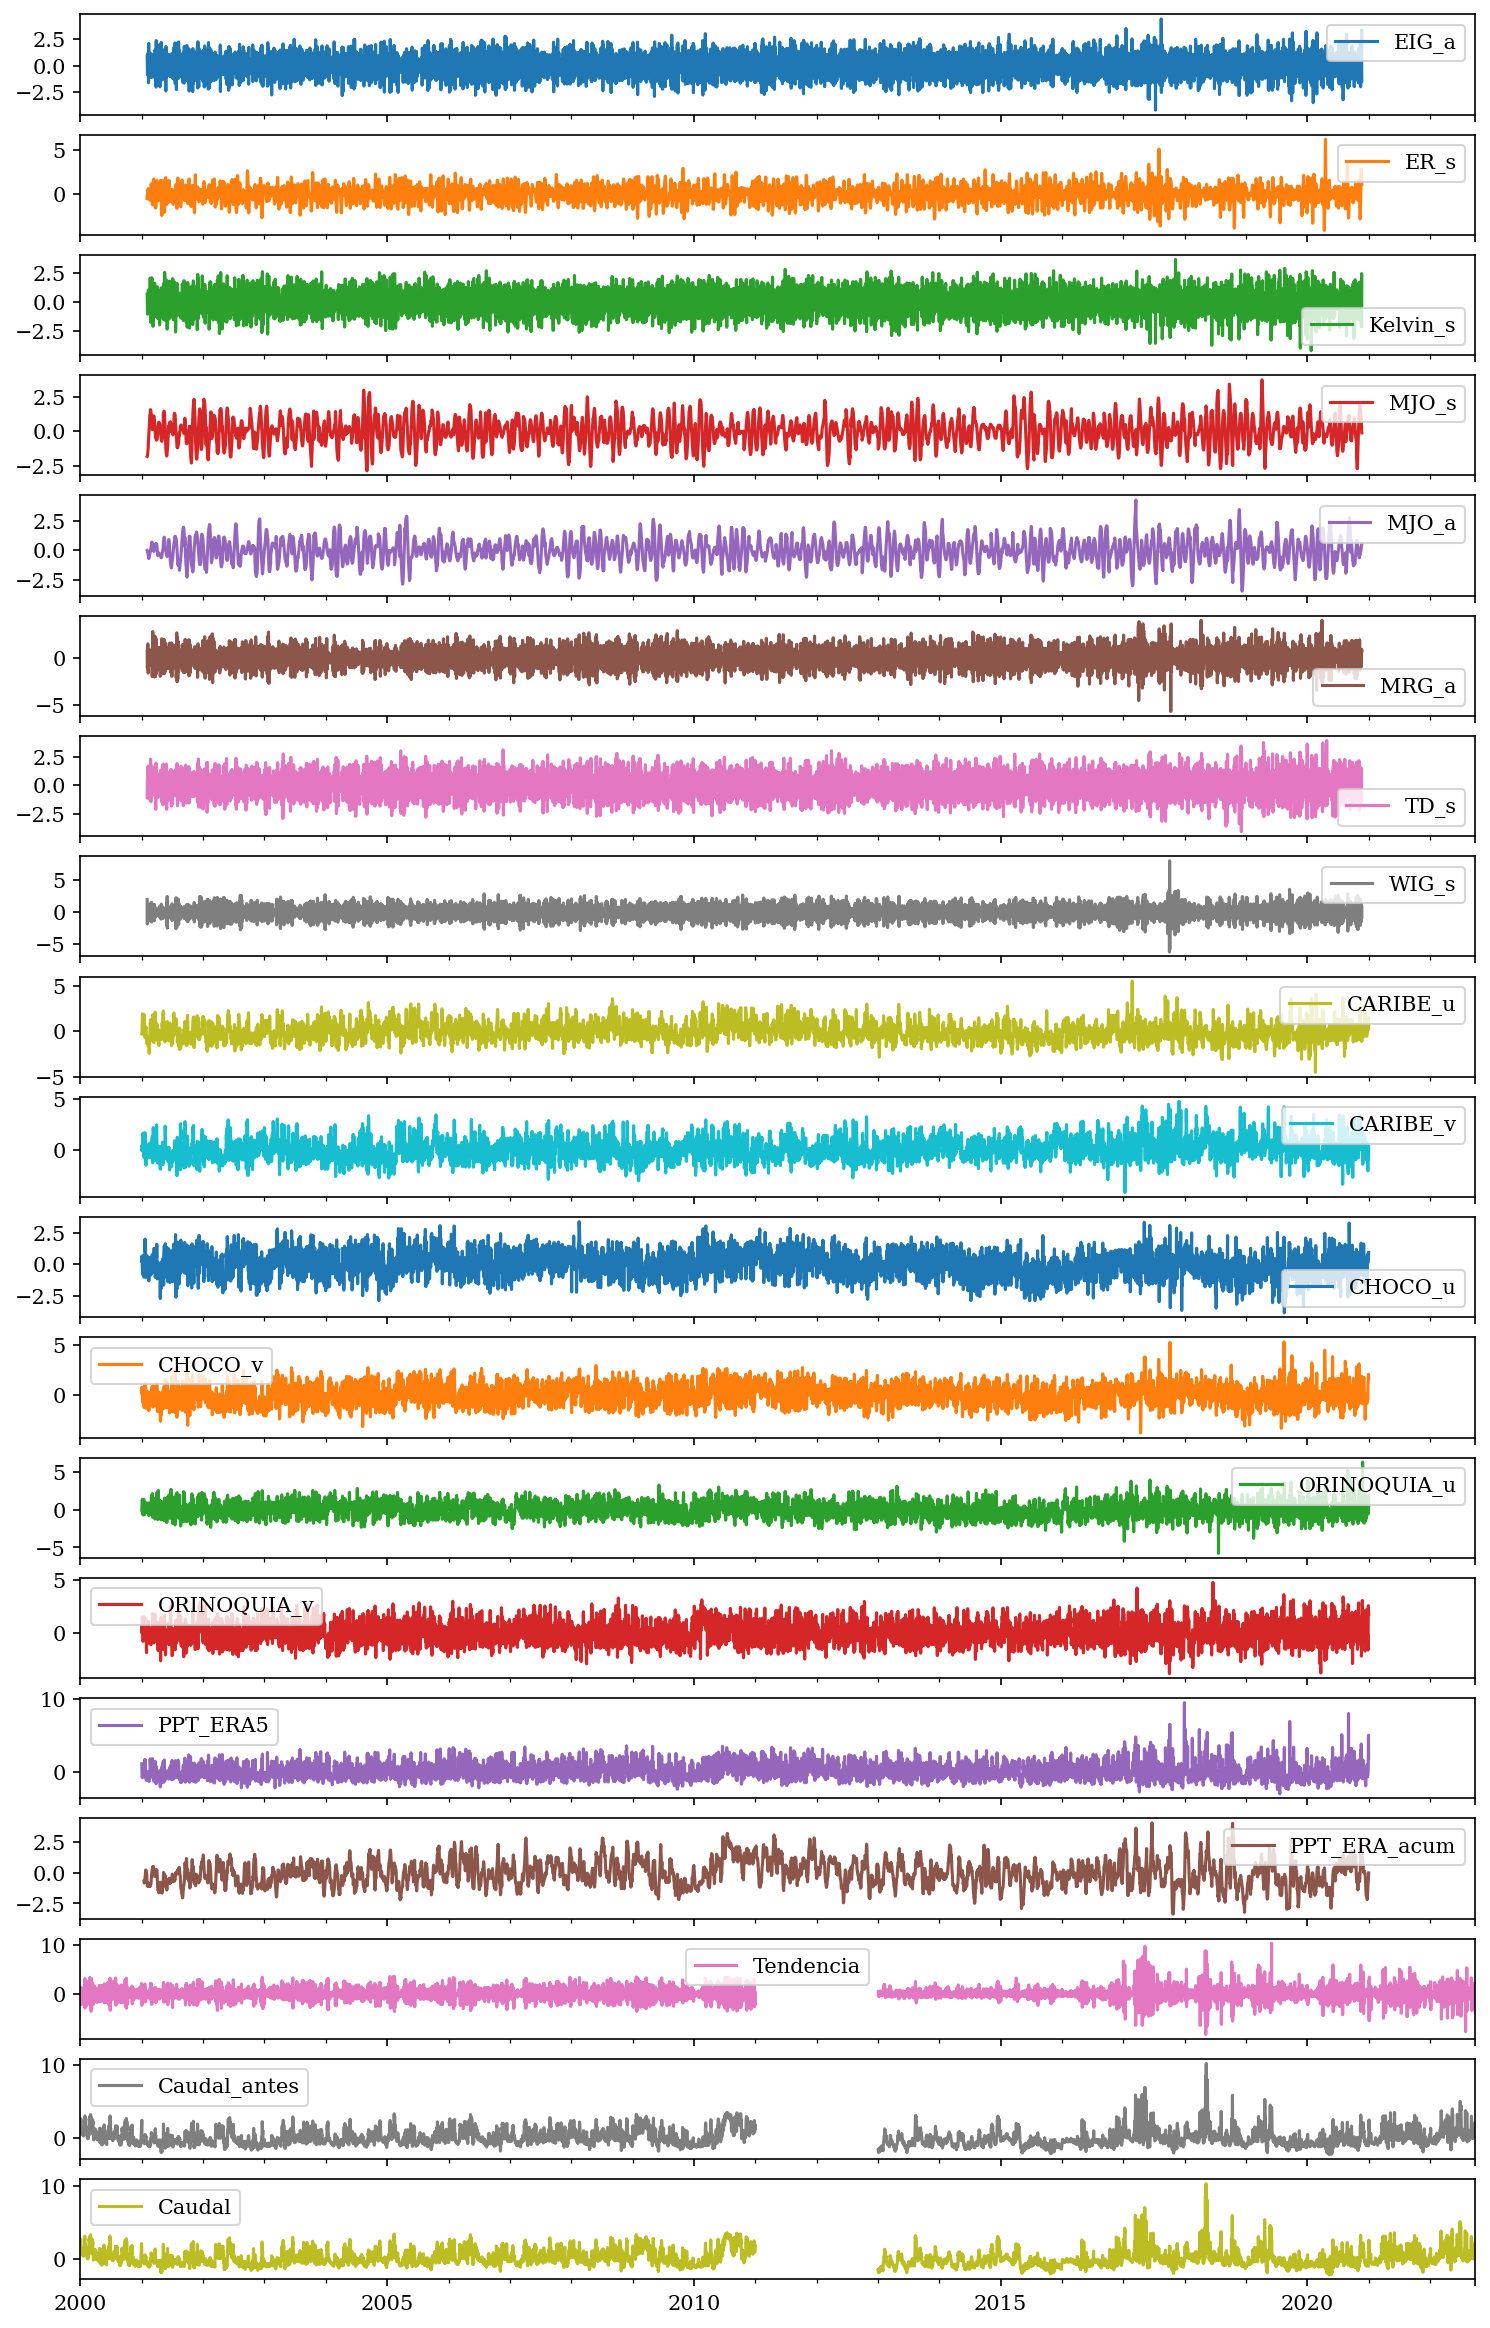
\includegraphics[width=0.85\textwidth]{G:/My Drive/Maestría en Recursos Hidraulicos/IA y AU en geociencias/Trabajo_final/Imagenes/Anomalias_estandarizadas.png}
	\caption{Series de anomalías estandarizadas de cada una de las variables predictoras y objetivo.} \label{fig:series_estand}
\end{figure}

De  esta imagen se puede observar que las anomalías en el periodo de prueba presentan valores mayores a los encontrados en el periodo de entrenamiento en todas las variables, pero que se ve más marcado en las variables de caudal y precipitación. Además, también se observa que en variables como el caudal se presentan variaciones interanuales.

Por otro lado, es bien sabido que cuando hablamos de pronósticos de series de tiempo, las relaciones entre las variables explicativas respecto a la variable objetivo pueden tener cierto rezago, por lo que se hace necesario desarrollar una analisis de correlaciones rezagadas con cada uno de los índices para determinar cuales son los rezagos óptimos para las variables que ingresan a los modelos. En este sentido, en la Figura \ref{fig:corr_resa} se presentan las correlaciones rezagadas de cada una de las variables con la variable objetivo. Se puede observar que las variables de la precipitación, las ondas kelvin, MRG y TD,  el chorro del caribe zonal y los chorros del chocó tienen un rezago de 1 día; Los chorros del chocó, y las ondas Rossby, tienen rezago de 2 y el chorro de la orinoquia rezago de 3; y además, variables tienen las mayores correlaciones con rezago 0, destacablemente el caudal del día antes y la precipitación acumulada. También es importante mencionar que estos rezagos por ejemplo en la precipitación son congruentes con el tiempo de concentración de la cuenca que es aproximadamente de 1.5 días.

\begin{figure}[!]
	\centering%
	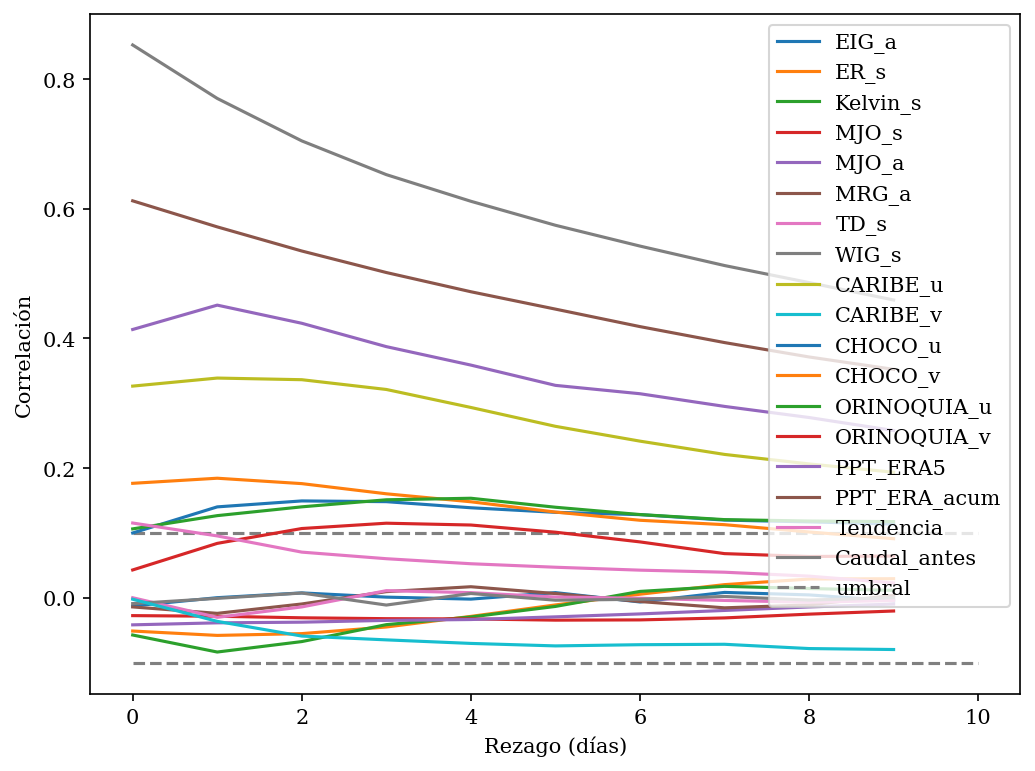
\includegraphics[width=0.8\textwidth]{G:/My Drive/Maestría en Recursos Hidraulicos/IA y AU en geociencias/Trabajo_final/Imagenes/Seleccion_rezago.png}
	\caption{Correlaciones rezagadas entre las variables explicativas y objetivo.} \label{fig:corr_resa}
\end{figure}

Con base en los rezagos anteriores se calculan las correlaciones entre los indices y las anomalías de caudal, donde resaltan altas correlaciones con el las anomalías de caudal antecedente (0.85), precipitación acumulada (0.61), precipitación del día anterior (0.45), caribe zonal con rezago 1 (0.31), entre otros, pero además se presentan altas relaciones entre las variables predictoras como las anomalías de caudal antecedente y la precipitación.  

En este sentido, se decide realizar un analisis de componentes principales con estas variables para obtener variables independientes entre ellas, que ingresen a los modelos de pronostico. En la Figura \ref{fig:corr_pcs} la matriz de correlación de las 18 componentes principales con las anomalías de caudal. Se puede observar que las componentes principales PC1, PC2, PC18, PC9, PC6, PC16, PC7 y PC8 superan el umbral de 0.1 de correlación y por tanto serán las variables que se utilizarán como variables predictoras en los modelos. Estas variables presentan una buena separación de las anomalías de caudal como se puede observar en la Figura \ref{fig:pc1pc2}, dónde en el espacio de las componentes principales PC1 y PC2, para valores negativos de ambas variables se tienen anomalías negativas de caudal, y para valores positivos de ambas variables se tienen anomalías positivas de caudal.

\begin{figure}[!]
	\centering%
	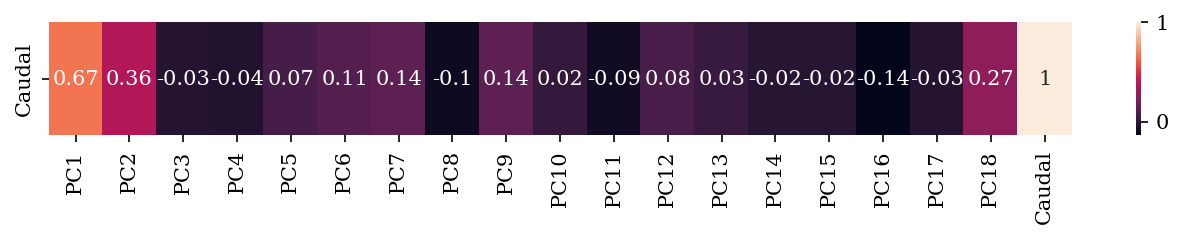
\includegraphics[width=0.8\textwidth]{G:/My Drive/Maestría en Recursos Hidraulicos/IA y AU en geociencias/Trabajo_final/Imagenes/Correlaciones_con_pcs.png}
	\caption{Correlaciones rezagadas entre las pcs y la variable objetivo.} \label{fig:corr_pcs}
\end{figure}


\begin{figure}[!]
	\centering%
	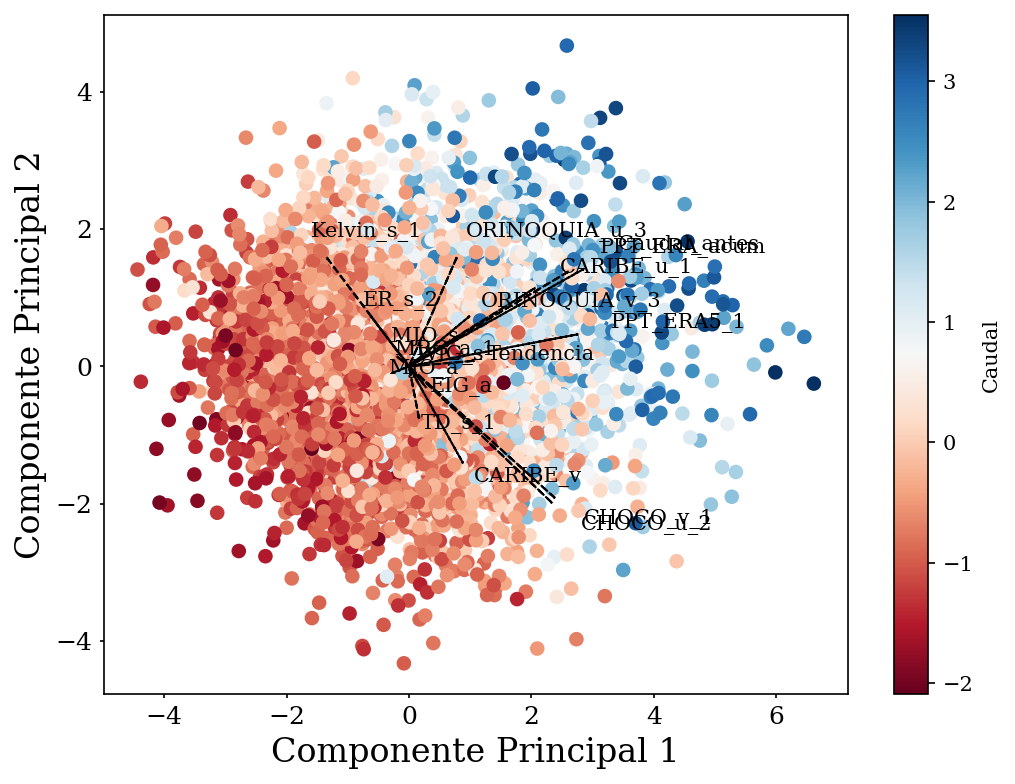
\includegraphics[width=0.5\textwidth]{G:/My Drive/Maestría en Recursos Hidraulicos/IA y AU en geociencias/Trabajo_final/Imagenes/PC1_PC2.png}
	\caption{Anomalías de caudal en el espacio de las PC1 y PC2.} \label{fig:pc1pc2}
\end{figure}


\subsection{Entrenamiento, validación y prueba de modelos}

De acuerdo con las variables definidas en la subsección anterior se plantean 7 modelos de pronostico a ser evaluados, estos son: regresión lineal múltiple (LR), vecino más cercano (KNN) con un tamaño de hojas igual a 1, nemero de vecinos cercanos de 21 y distancia de Manhattan; vectores de soporte (SVR) cn parametros X=6.67, gamma=0.01 y kernel lineal; ramdom forest (RF) con 800 estimadores, separaciones se muestras minimas de 2 y profundidad mínima de 100; SARIMAX con p=2 y q=1;  redes neurales artificiales tipo percertrón multicapa (MLP) con 3 capas de 10,10 y 50 neuronas y una función de activación tangente hiperbólica; redes neuronales recurrentes de largo y corto plazo (LSTM) con las 3 capas de 10,10 y 50 neuronas cada una con una capa de dropout de 0.1. Todos estos modelos, excpecto SARIMAX y LSTM, se evaluan en el periodo de entrenamiento por medio de una validación cruzada kfold de ventanas sucesivas y la métrica del r2, y además, se presenta la curva de entrenamiento para determinar si es posible que el modelo continué aprendiendo de más datos. 

En la Figura \ref{fig:kfold} se pueden observar la validación cruzada de los modelos en la cual la forma de la función es similar en todos los modelos, donde se presenta un mejor desempeño en la ventana 4 de validación, del orden de 0.8. Además, los desempeños en las demás ventanas son del orden de 0.6, aunque con mejores resultados en la regresión lineal, la red neuronal MLP y SVR. Dado que estos tres modelos presentan resultados similares, se calculan las curvas de aprendizaje que se presentan en la Figura \ref{fig:LC}, de donde se puede observar que el modelo de regresión lineal y SVR aunque presentan buen desempeño, las curvas muestran que no pueden aprender más, mientras la red neuronal podría seguir aprendiendo con más muestras. Asimismo, se observa problemas de varianza en RF y KNN, siendo el primero más critico.

\begin{figure}[!]
	\centering%
	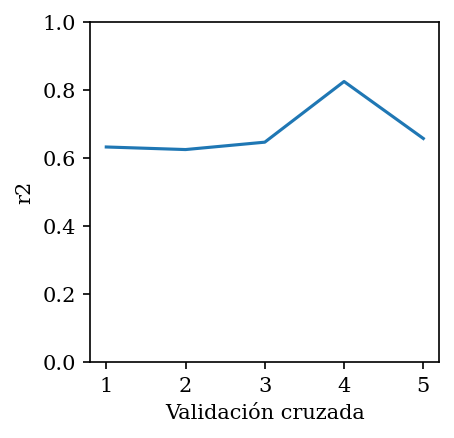
\includegraphics[width=0.3\textwidth]{G:/My Drive/Maestría en Recursos Hidraulicos/IA y AU en geociencias/Trabajo_final/Imagenes/R_LR_CV_r2.png}
	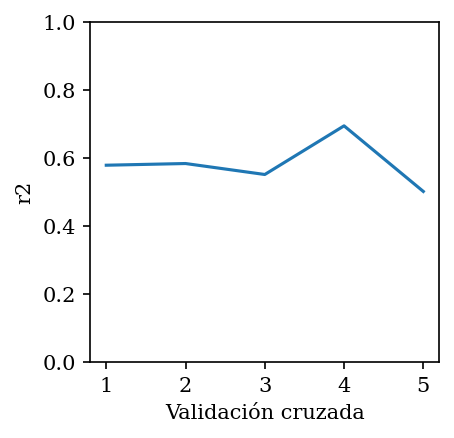
\includegraphics[width=0.3\textwidth]{G:/My Drive/Maestría en Recursos Hidraulicos/IA y AU en geociencias/Trabajo_final/Imagenes/R_KNN_CV_r2.png}
	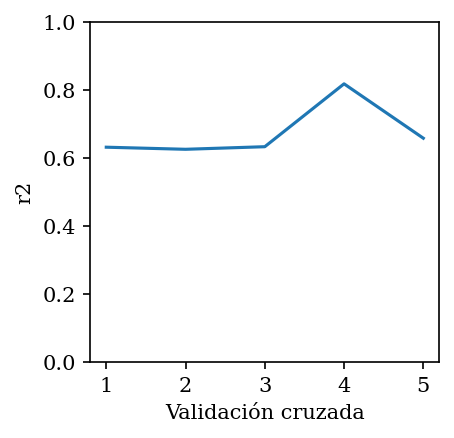
\includegraphics[width=0.3\textwidth]{G:/My Drive/Maestría en Recursos Hidraulicos/IA y AU en geociencias/Trabajo_final/Imagenes/R_SVR_CV_r2.png}\\
	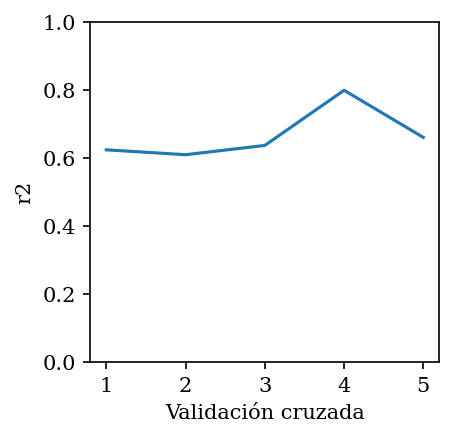
\includegraphics[width=0.3\textwidth]{G:/My Drive/Maestría en Recursos Hidraulicos/IA y AU en geociencias/Trabajo_final/Imagenes/R_MLP_CV_r2.png}
	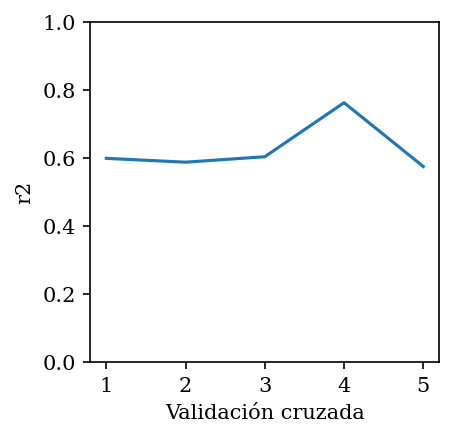
\includegraphics[width=0.3\textwidth]{G:/My Drive/Maestría en Recursos Hidraulicos/IA y AU en geociencias/Trabajo_final/Imagenes/R_RF_CV_r2.png}
	\caption{Validación cruzada en términos del r2 para los modelos de LR, KNN, SVR, MLP y RF (de izquierda a derecha y arriba hacia abajo).} \label{fig:kfold}
\end{figure}


\begin{figure}[!]
	\centering%
	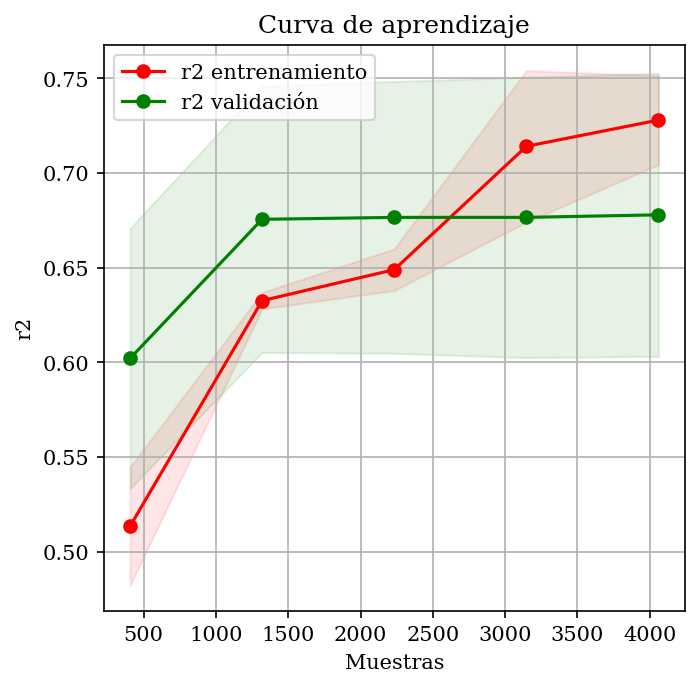
\includegraphics[width=0.3\textwidth]{G:/My Drive/Maestría en Recursos Hidraulicos/IA y AU en geociencias/Trabajo_final/Imagenes/R_LR_LC_r2.png}
	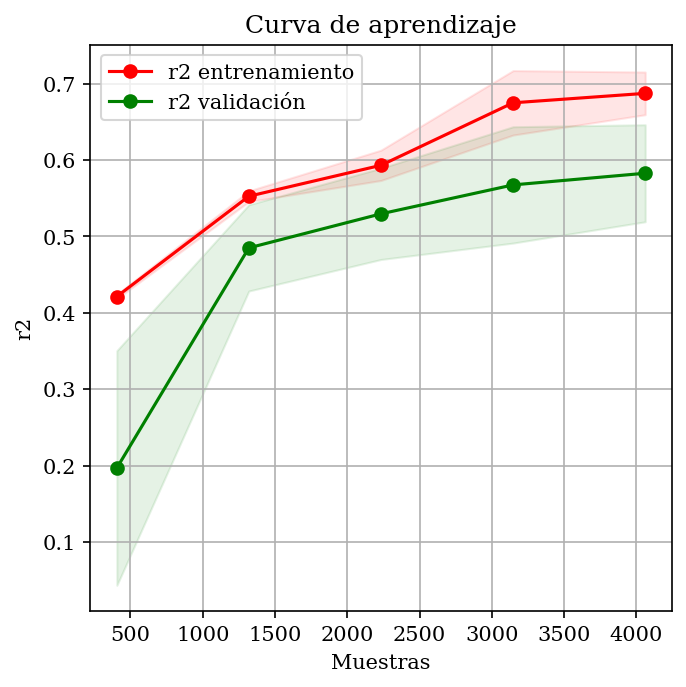
\includegraphics[width=0.3\textwidth]{G:/My Drive/Maestría en Recursos Hidraulicos/IA y AU en geociencias/Trabajo_final/Imagenes/R_KNN_LC_r2.png}
	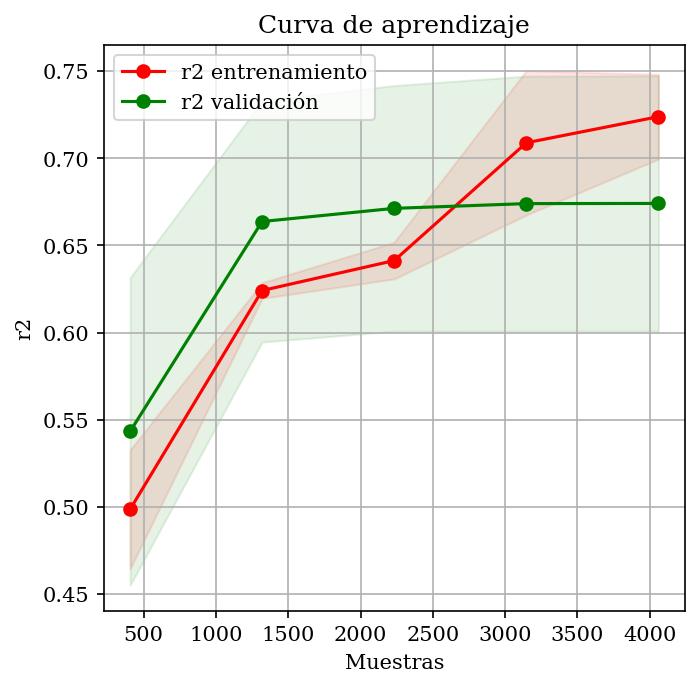
\includegraphics[width=0.3\textwidth]{G:/My Drive/Maestría en Recursos Hidraulicos/IA y AU en geociencias/Trabajo_final/Imagenes/R_SVR_LC_r2.png}\\
	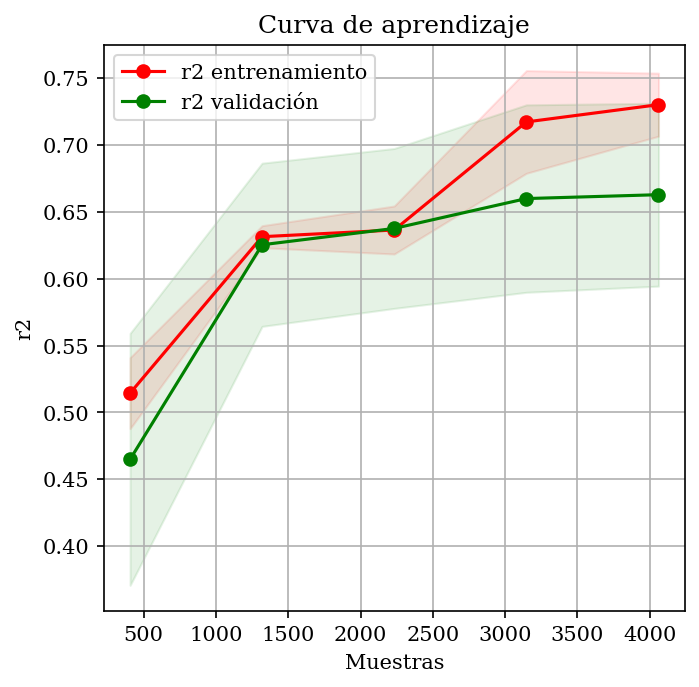
\includegraphics[width=0.3\textwidth]{G:/My Drive/Maestría en Recursos Hidraulicos/IA y AU en geociencias/Trabajo_final/Imagenes/R_MLP_LC_r2.png}
	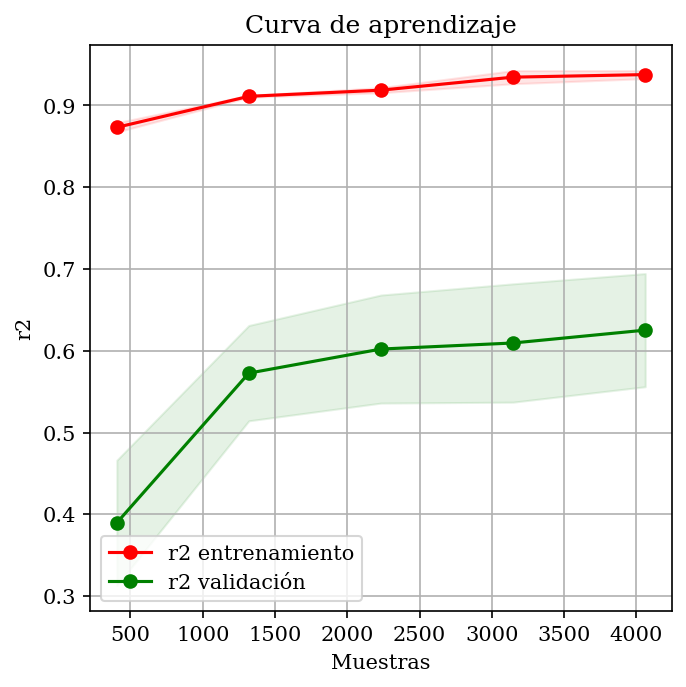
\includegraphics[width=0.3\textwidth]{G:/My Drive/Maestría en Recursos Hidraulicos/IA y AU en geociencias/Trabajo_final/Imagenes/R_RF_LC_r2.png}
	\caption{Curva de aprendizaje en términos del r2 para los modelos de LR, KNN, SVR, MLP y RF (de izquierda a derecha y arriba hacia abajo).} \label{fig:LC}
\end{figure}

Por otro lado, dado que el modelo SARIMAX y LSTM requieren de continuidad porque son modelos que guardan memoria, estos se calibraron desde 2013 hasta 2016. Los resultados de la distribución de los residuales del modelo SARIMAX es similar al de regresión lineal, donde ambos se distribuyen de manera normal con algunos alejamientos en los eventos extremos. Asimismo, el modelo corrido para LSTM, muestra que no podría seguir aprendiendo con los hiperparametros que se le han sobreimpuesto.

Para evaluar equitativamente el desempeño de los modelos se pronostican las anomalías de caudal en el periodo de prueba (2017-2020) y se calcula las métricas de r2 y error cuadrático medio (mse), las cuales se consignan en la Figura \ref{fig:test_r2_mse}. Se puede observar que de acuerdo con estas métricas, los mejores 4 modelos en orden decendente son MLP, SARIMAX, LR y SVR, que son los mismos modelos en lo que el desempeño en el entrenamiento era superior. 

\begin{figure}[!]
	\centering%
	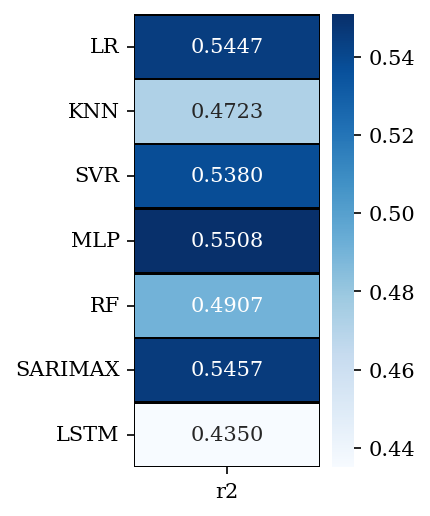
\includegraphics[width=0.3\textwidth]{G:/My Drive/Maestría en Recursos Hidraulicos/IA y AU en geociencias/Trabajo_final/Imagenes/r2_anomalias.png}
	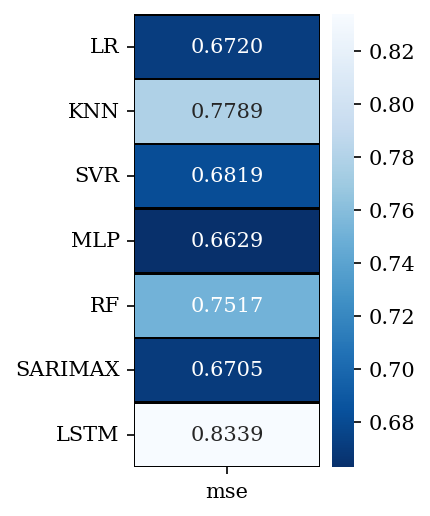
\includegraphics[width=0.3\textwidth]{G:/My Drive/Maestría en Recursos Hidraulicos/IA y AU en geociencias/Trabajo_final/Imagenes/mse_anomalias.png}
	\caption{Curva de aprendizaje en términos del r2 para los modelos de LR, KNN, SVR, MLP y RF (de izquierda a derecha y arriba hacia abajo).} \label{fig:test_r2_mse}
\end{figure}

\subsection{Ganancia respecto a pronósticos de referencia}

Pronosticar las anomalías de caudal surgió como una necesidad debido a que las variables climáticas tienen un marcado ciclo anual. En este punto, es necesario desestandarizar las anomalías de caudal, es decir, volver a las unidades originales del caudal para determinar el valor real del pronostico. En la Figura \ref{fig:series_pron} se presenta los pronósticos de cada modelo, junto con el caudal observado y la climatología. Se puede observar que las deficiencias en algunos modelos como KNN que presentan bajos desempeños se debe a que los picos más altos no son alcanzados y estos pesan más en el error. 

También se observa que modelos como LSTM captura los extremos pero se equivoca más en otros rangos de valores, pero en general, se ve una representación de los caudales mayor que la climatología, pero para evaluar esto más contundente mente en la Figura \ref{fig:SS} se presenta la métrica de ganancia con respecto a la climatología y al caudal antecedente. De esta ultima figura, se observa que los mejores modelos son consistentes con los encontrados anteriormente para representar las anomalías de caudal. Por ejemplo, el modelo de redes neuronales MLP presenta un 50\% de ganancia respecto a pronosticar con la climatología y un 14\% respecto a pronósticar con el caudal del día anterior, asimismo, el modelo SARIMAX tiene un comportamiento similar con un 12.4\% de ganancia con respecto al caudal del día anterior, y los modelos de LR y SVR comprenden también ganancia del 49\% respecto a la climatología y 12\% y 10\% respecto al caudal del día anterior, respectivamente. Es de notar también que el modelo LSTM, a pesar de que presenta ganancias con respecto a la climatología, su desempeño es menor que el del pronostico antecedente, lo cual podría indicar que para este modelo su solución optima se encuentra en otro dominio de parámetros, dado que si captura correctamente los extremos.


\begin{figure}[!]
	\centering%
	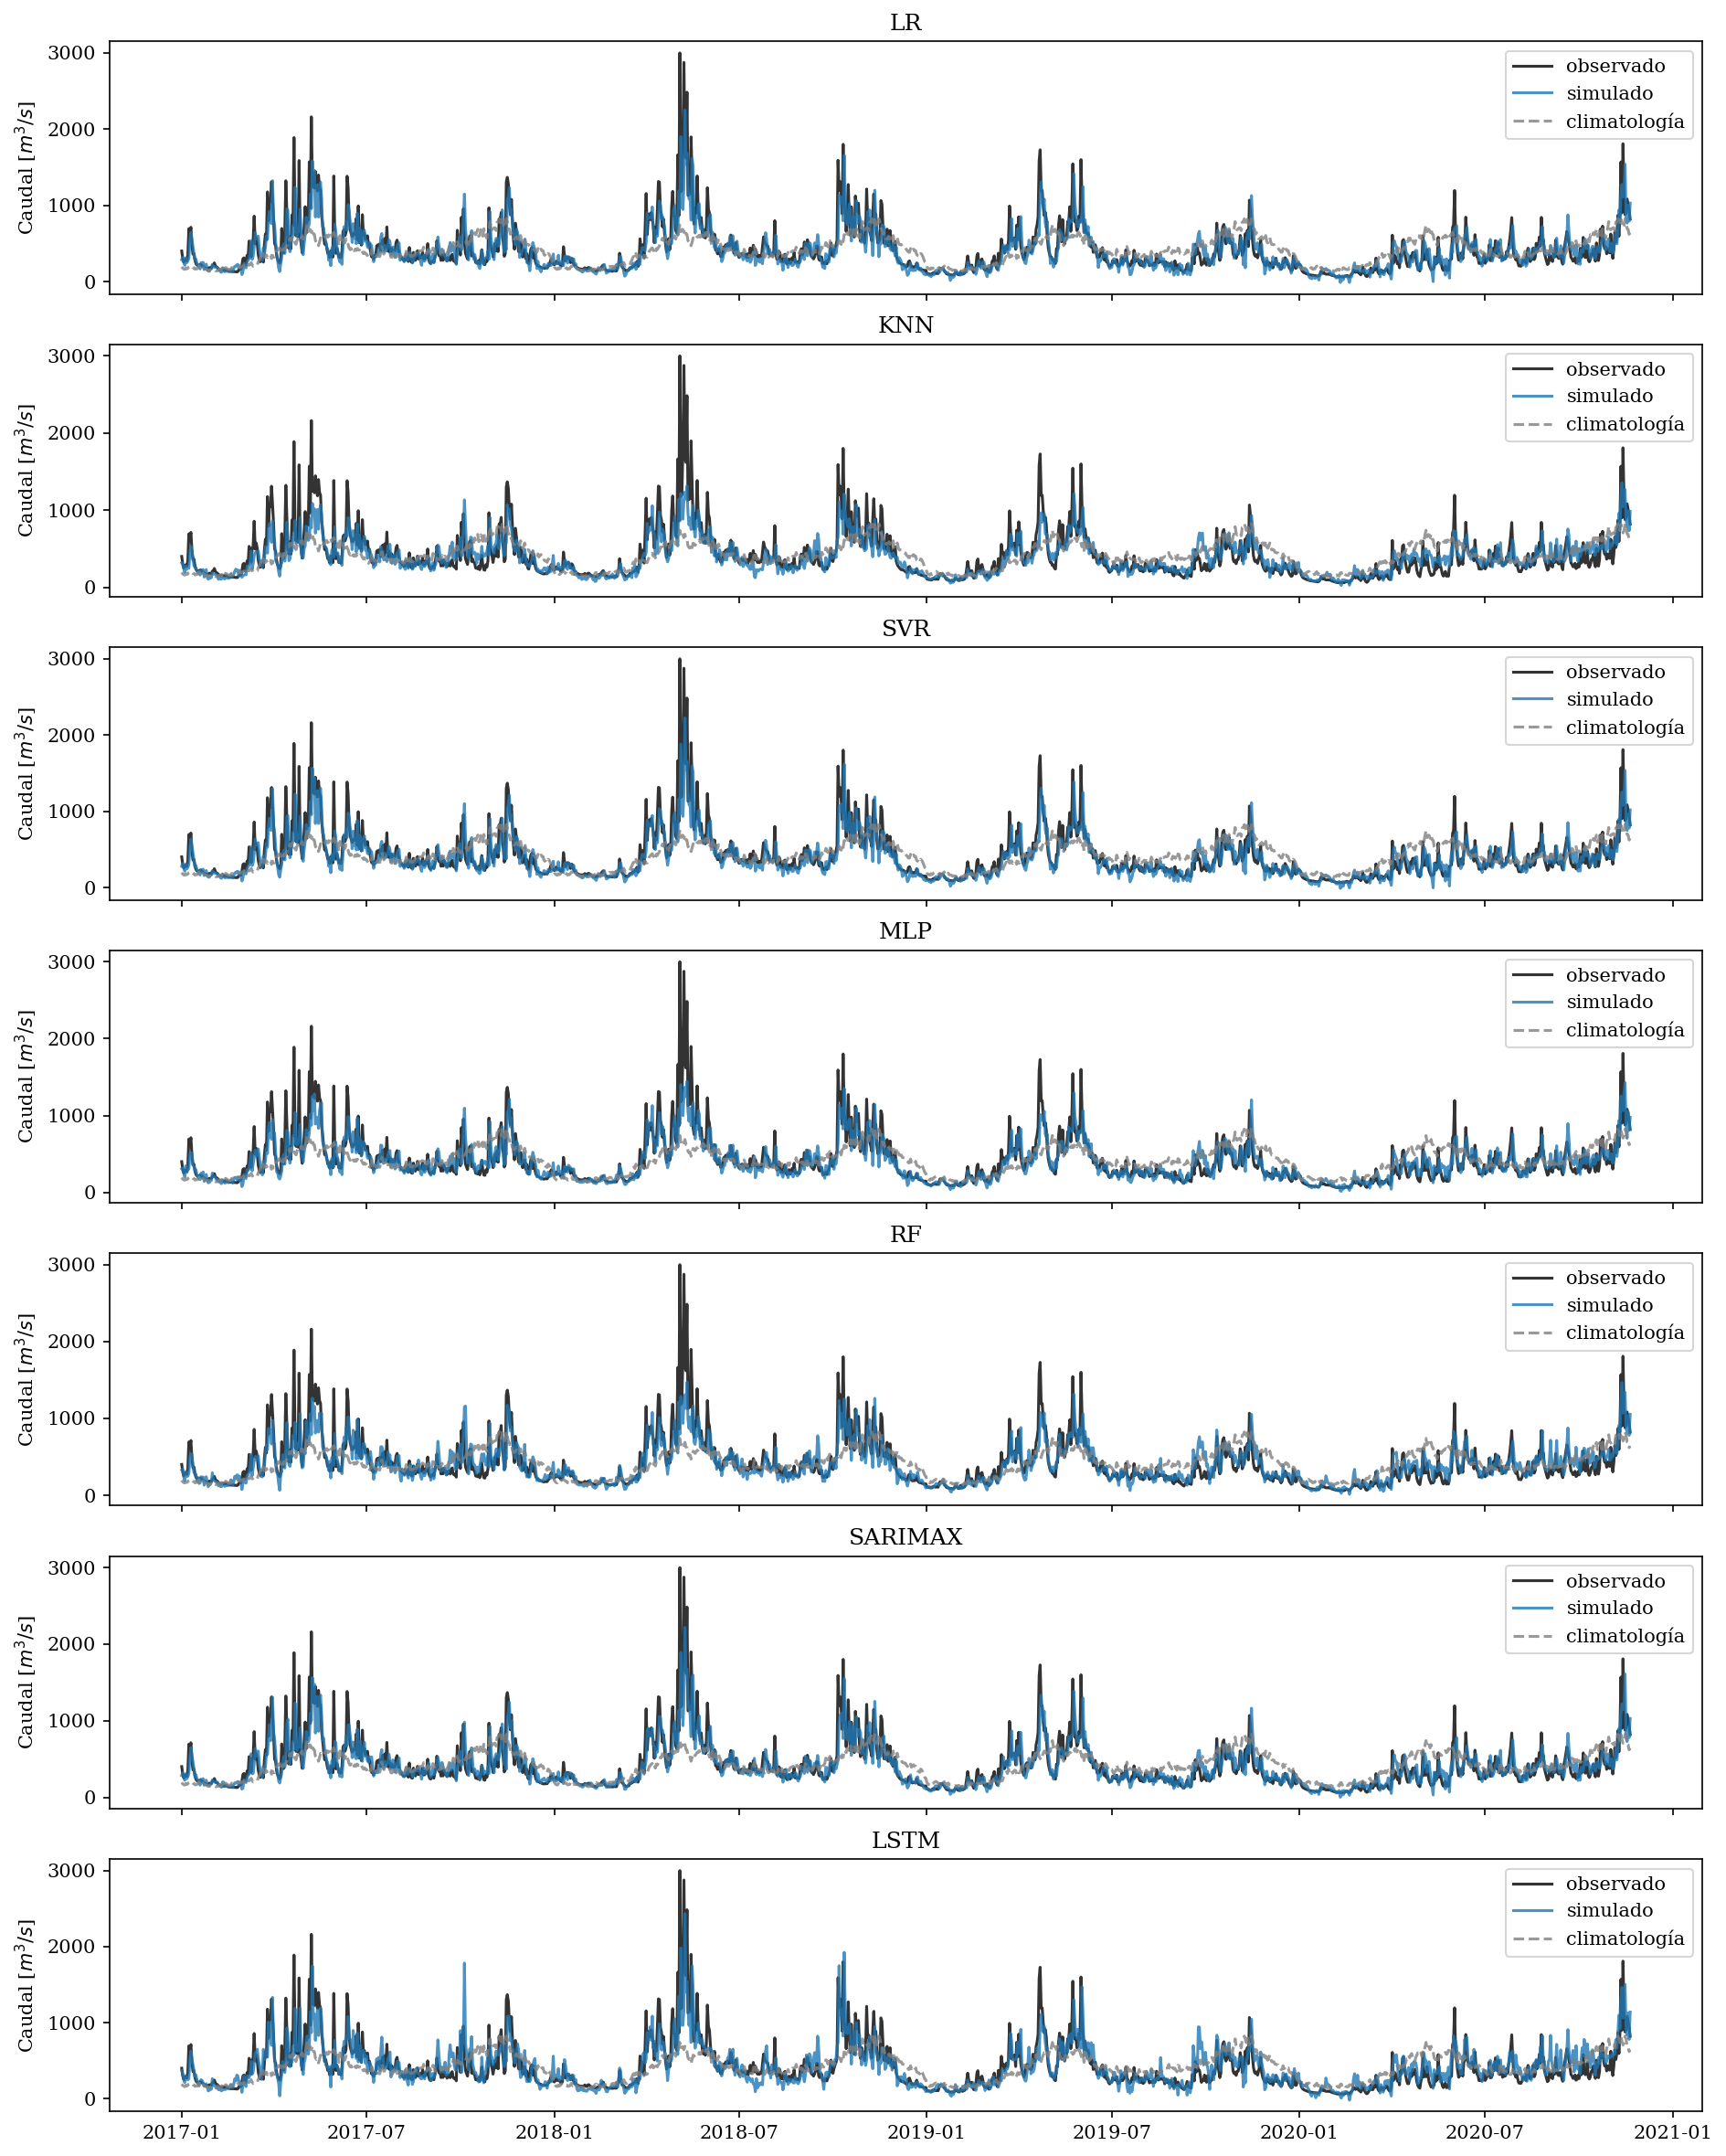
\includegraphics[width=1.0\textwidth]{G:/My Drive/Maestría en Recursos Hidraulicos/IA y AU en geociencias/Trabajo_final/Imagenes/pronosticos_series_modelos.png}
	\caption{Series pronosticadas por cada uno de los modelos en el periodo de prueba.} \label{fig:series_pron}
\end{figure}

\begin{figure}[!]
	\centering%
	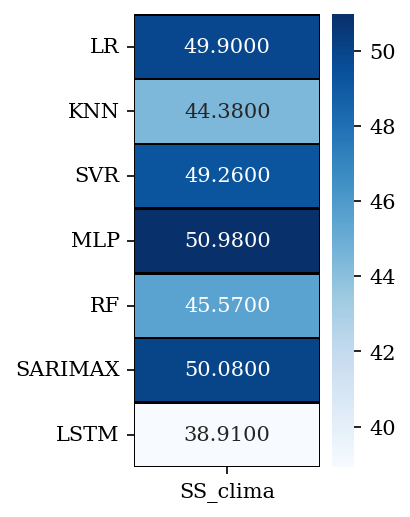
\includegraphics[width=0.3\textwidth]{G:/My Drive/Maestría en Recursos Hidraulicos/IA y AU en geociencias/Trabajo_final/Imagenes/SS_CLIMA.png}
	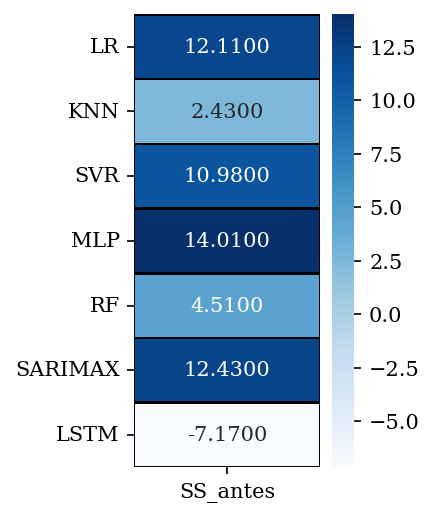
\includegraphics[width=0.3\textwidth]{G:/My Drive/Maestría en Recursos Hidraulicos/IA y AU en geociencias/Trabajo_final/Imagenes/SS_ANTES.png}
	\caption{Curva de aprendizaje en términos del r2 para los modelos de LR, KNN, SVR, MLP y RF (de izquierda a derecha y arriba hacia abajo).} \label{fig:SS}
\end{figure}


\section{Conclusiones}

El analisis de selección de variables permitió identificar que variables como el caudal antecedente y la precipitación acumulada en los últimos 7 días y del día anterior sobre la cuenca son las variables que más se correlacionan con las anomalías de caudal sobre la cuenca de Sogamoso, sin descartar que las otras variables también presentan correlaciones significativas. Pero además, estás variables también están correlacionadas entre sí, por lo cual, al aplicar el analisis de componentes principales se obtuvieron 18 componentes de las cuales 8 se correlacionan con las anomalías de caudal superando el umbral de 0.1 de correlación, lo cual permitió tener una adecuada reducción de dimensiones en el problema.

Del entrenamiento, validación y prueba de los modelos se pudo identificar que para este problema especifico los modelos que presentaron un mejor desempeño fueron LR, SVR, SARIMAX y MLP. Dónde, el modelo de regresión lineal y SVR presentan desempeños muy similares y se muestran limitados al seguir aprendiendo con base en más cantidad de muestras, mientras que por su lado, el modelo MLP muestra que tiene capacidad de seguir aprendiendo a medida que se aumente el numero de muestras para entrenar. En el periodo de prueba estos mismos modelos se siguieron destacando presentando un desempeño superior a KNN y RF, los cuales presentan problemas de varianza.

Por ultimo, la ganancia que tienen estos modelos con respecto a la climatología es notable, yendo desde 38\% hasta 50\% y siendo el modelo MLP el que presenta el mejor desempeño con 50.9\% de ganancia. Asimismo, este ultimo modelo presenta la mayor ganancia con respecto al pronostico antecedente, junto con SARIMAX, LR y SVR. Esto muestra, que este tipo de modelos estadísticos se pueden utilizar para pronosticar el caudal diario en cuencas como Sogamoso, lo cual puede repercutir en mejorar las regulación en este rio en el cual se tiene un embalse y se genera energía hidroeléctrica.

% \section{= enter section title =}
%Text here ===>>>


%%

%  Numbered lines in equations:
%  To add line numbers to lines in equations,
%  \begin{linenomath*}
%  \begin{equation}
%  \end{equation}
%  \end{linenomath*}



%% Enter Figures and Tables near as possible to where they are first mentioned:
%
% DO NOT USE \psfrag or \subfigure commands.
%
% Figure captions go below the figure.
% Table titles go above tables;  other caption information
%  should be placed in last line of the table, using
% \multicolumn2l{$^a$ This is a table note.}
%
%----------------
% EXAMPLE FIGURES
%
% \begin{figure}
% \includegraphics{example.png}
% \caption{caption}
% \end{figure}
%
% Giving latex a width will help it to scale the figure properly. A simple trick is to use \textwidth. Try this if large figures run off the side of the page.
% \begin{figure}
% \noindent\includegraphics[width=\textwidth]{anothersample.png}
%\caption{caption}
%\label{pngfiguresample}
%\end{figure}
%
%
% If you get an error about an unknown bounding box, try specifying the width and height of the figure with the natwidth and natheight options. This is common when trying to add a PDF figure without pdflatex.
% \begin{figure}
% \noindent\includegraphics[natwidth=800px,natheight=600px]{samplefigure.pdf}
%\caption{caption}
%\label{pdffiguresample}
%\end{figure}
%
%
% PDFLatex does not seem to be able to process EPS figures. You may want to try the epstopdf package.
%

%
% ---------------
% EXAMPLE TABLE
% Please do NOT include vertical lines in tables
% if the paper is accepted, Wiley will replace vertical lines with white space
% the CLS file modifies table padding and vertical lines may not display well
%
% \begin{table}
% \caption{Time of the Transition Between Phase 1 and Phase 2$^{a}$}
% \centering
% \begin{tabular}{l c}
% \hline
%  Run  & Time (min)  \\
% \hline
%   $l1$  & 260   \\
%   $l2$  & 300   \\
%   $l3$  & 340   \\
%   $h1$  & 270   \\
%   $h2$  & 250   \\
%   $h3$  & 380   \\
%   $r1$  & 370   \\
%   $r2$  & 390   \\
% \hline
% \multicolumn{2}{l}{$^{a}$Footnote text here.}
% \end{tabular}
% \end{table}

%% SIDEWAYS FIGURE and TABLE
% AGU prefers the use of {sidewaystable} over {landscapetable} as it causes fewer problems.
%
% \begin{sidewaysfigure}
% \includegraphics[width=20pc]{figsamp}
% \caption{caption here}
% \label{newfig}
% \end{sidewaysfigure}
%
%  \begin{sidewaystable}
%  \caption{Caption here}
% \label{tab:signif_gap_clos}
%  \begin{tabular}{ccc}
% one&two&three\\
% four&five&six
%  \end{tabular}
%  \end{sidewaystable}

%% If using numbered lines, please surround equations with \begin{linenomath*}...\end{linenomath*}
%\begin{linenomath*}
%\begin{equation}
%y|{f} \sim g(m, \sigma),
%\end{equation}
%\end{linenomath*}

%%% End of body of article

%%%%%%%%%%%%%%%%%%%%%%%%%%%%%%%%
%% Optional Appendix goes here
%
% The \appendix command resets counters and redefines section heads
%
% After typing \appendix
%
%\section{Here Is Appendix Title}
% will show
% A: Here Is Appendix Title
%
%\appendix
%\section{Here is a sample appendix}

%%%%%%%%%%%%%%%%%%%%%%%%%%%%%%%%%%%%%%%%%%%%%%%%%%%%%%%%%%%%%%%%
%
% Optional Glossary, Notation or Acronym section goes here:
%
%%%%%%%%%%%%%%
% Glossary is only allowed in Reviews of Geophysics
%  \begin{glossary}
%  \term{Term}
%   Term Definition here
%  \term{Term}
%   Term Definition here
%  \term{Term}
%   Term Definition here
%  \end{glossary}

%
%%%%%%%%%%%%%%
% Acronyms
%   \begin{acronyms}
%   \acro{Acronym}
%   Definition here
%   \acro{EMOS}
%   Ensemble model output statistics
%   \acro{ECMWF}
%   Centre for Medium-Range Weather Forecasts
%   \end{acronyms}

%
%%%%%%%%%%%%%%
% Notation
%   \begin{notation}
%   \notation{$a+b$} Notation Definition here
%   \notation{$e=mc^2$}
%   Equation in German-born physicist Albert Einstein's theory of special
%  relativity that showed that the increased relativistic mass ($m$) of a
%  body comes from the energy of motion of the body—that is, its kinetic
%  energy ($E$)—divided by the speed of light squared ($c^2$).
%   \end{notation}



%\section{Open Research}
%AGU requires an Availability Statement for the underlying data needed to understand, evaluate, and build upon the reported research at the time of peer review and publication.
%
%Authors should include an Availability Statement for the software that has a significant impact on the research. Details and templates are in the Availability Statement section of the Data and Software for Authors Guidance: \url{https://www.agu.org/Publish-with-AGU/Publish/Author-Resources/Data-and-Software-for-Authors#availability}
%
%It is important to cite individual datasets in this section and, and they must be included in your bibliography. Please use the type field in your bibtex file to specify the type of data cited. Options include [Dataset], [Software], [ComputationalNotebook], [Collection].
%Example:
%
%@misc{https://doi.org/10.7283/633e-1497,
%  doi = {10.7283/633E-1497},
%  url = {https://www.unavco.org/data/doi/10.7283/633E-1497},
%  author = {de Zeeuw-van Dalfsen, Elske and Sleeman, Reinoud},
%  title = {KNMI Dutch Antilles GPS Network - SAB1-St_Johns_Saba_NA P.S.},
%  publisher = {UNAVCO, Inc.},
%  year = {2019},
%  type = {dataset}
%}

%
%For physical samples, use the IGSN persistent identifier, see the International Geo Sample Numbers section:
%\url{https://www.agu.org/Publish-with-AGU/Publish/Author-Resources/Data-and-Software-for-Authors#IGSN}
%%%%%%%%%%%%%%%%%%%%%%%%%%%%%%%%%%%%%%%%%%%%%%%%
%
%\acknowledgments
%This section is optional. Include any Acknowledgments here.
%The acknowledgments should list:\\
%All funding sources related to this work from all authors\\
%Any real or perceived financial conflicts of interests for any author\\
%Other affiliations for any author \newline that may be perceived as having a conflict of interest with respect to the results of this paper.\\
%\clearpage
%It is also the appropriate place to thank colleagues and other contributors. AGU does not normally allow dedications.\\
%%\input{methods}
%Hello here is some text in Nick's file
%\input{data}


%% ------------------------------------------------------------------------ %%
%% References and Citations

%%%%%%%%%%%%%%%%%%%%%%%%%%%%%%%%%%%%%%%%%%%%%%%
%
% \bibliography{<name of your .bib file>} don't specify the file extension
%
% don't specify bibliographystyle

% In the References section, cite the data/software described in the Availability Statement (this includes primary and processed data used for your research). For details on data/software citation as well as examples, see the Data & Software Citation section of the Data & Software for Authors guidance
% https://www.agu.org/Publish-with-AGU/Publish/Author-Resources/Data-and-Software-for-Authors#citation

%%%%%%%%%%%%%%%%%%%%%%%%%%%%%%%%%%%%%%%%%%%%%%%

\bibliography{bibliography}

%Reference citation instructions and examples:
%
% Please use ONLY \cite and \citeA for reference citations.
% \cite for parenthetical references
% ...as shown in recent studies (Simpson et al., 2019)
% \citeA for in-text citations
% ...Simpson et al. (2019) have shown...
%
%
%...as shown by \citeA{jskilby}.
%...as shown by \citeA{lewin76}, \citeA{carson86}, \citeA{bartoldy02}, and \citeA{rinaldi03}.
%...has been shown \cite{jskilbye}.
%...has been shown \cite{lewin76,carson86,bartoldy02,rinaldi03}.
%... \cite <i.e.>[]{lewin76,carson86,bartoldy02,rinaldi03}.
%...has been shown by \cite <e.g.,>[and others]{lewin76}.
%
% apacite uses < > for prenotes and [ ] for postnotes
% DO NOT use other cite commands (e.g., \citet, \citep, \citeyear, \citealp, etc.).
% \nocite is okay to use to add references from your Supporting Information
%



\end{document}



More Information and Advice:

%% ------------------------------------------------------------------------ %%
%
%  SECTION HEADS
%
%% ------------------------------------------------------------------------ %%

% Capitalize the first letter of each word (except for
% prepositions, conjunctions, and articles that are
% three or fewer letters).

% AGU follows standard outline style; therefore, there cannot be a section 1 without
% a section 2, or a section 2.3.1 without a section 2.3.2.
% Please make sure your section numbers are balanced.
% ---------------
% Level 1 head
%
% Use the \section{} command to identify level 1 heads;
% type the appropriate head wording between the curly
% brackets, as shown below.
%
%An example:
%\section{Level 1 Head: Introduction}
%
% ---------------
% Level 2 head
%
% Use the \subsection{} command to identify level 2 heads.
%An example:
%\subsection{Level 2 Head}
%
% ---------------
% Level 3 head
%
% Use the \subsubsection{} command to identify level 3 heads
%An example:
%\subsubsection{Level 3 Head}
%
%---------------
% Level 4 head
%
% Use the \subsubsubsection{} command to identify level 3 heads
% An example:
%\subsubsubsection{Level 4 Head} An example.
%
%% ------------------------------------------------------------------------ %%
%
%  IN-TEXT LISTS
%
%% ------------------------------------------------------------------------ %%
%
% Do not use bulleted lists; enumerated lists are okay.
% \begin{enumerate}
% \item
% \item
% \item
% \end{enumerate}
%
%% ------------------------------------------------------------------------ %%
%
%  EQUATIONS
%
%% ------------------------------------------------------------------------ %%

% Single-line equations are centered.
% Equation arrays will appear left-aligned.

Math coded inside display math mode \[ ...\]
 will not be numbered, e.g.,:
 \[ x^2=y^2 + z^2\]

 Math coded inside \begin{equation} and \end{equation} will
 be automatically numbered, e.g.,:
 \begin{equation}
 x^2=y^2 + z^2
 \end{equation}


% To create multiline equations, use the
% \begin{eqnarray} and \end{eqnarray} environment
% as demonstrated below.
\begin{eqnarray}
  x_{1} & = & (x - x_{0}) \cos \Theta \nonumber \\
        && + (y - y_{0}) \sin \Theta  \nonumber \\
  y_{1} & = & -(x - x_{0}) \sin \Theta \nonumber \\
        && + (y - y_{0}) \cos \Theta.
\end{eqnarray}

%If you don't want an equation number, use the star form:
%\begin{eqnarray*}...\end{eqnarray*}

% Break each line at a sign of operation
% (+, -, etc.) if possible, with the sign of operation
% on the new line.

% Indent second and subsequent lines to align with
% the first character following the equal sign on the
% first line.

% Use an \hspace{} command to insert horizontal space
% into your equation if necessary. Place an appropriate
% unit of measure between the curly braces, e.g.
% \hspace{1in}; you may have to experiment to achieve
% the correct amount of space.


%% ------------------------------------------------------------------------ %%
%
%  EQUATION NUMBERING: COUNTER
%
%% ------------------------------------------------------------------------ %%

% You may change equation numbering by resetting
% the equation counter or by explicitly numbering
% an equation.

% To explicitly number an equation, type \eqnum{}
% (with the desired number between the brackets)
% after the \begin{equation} or \begin{eqnarray}
% command.  The \eqnum{} command will affect only
% the equation it appears with; LaTeX will number
% any equations appearing later in the manuscript
% according to the equation counter.
%

% If you have a multiline equation that needs only
% one equation number, use a \nonumber command in
% front of the double backslashes (\\) as shown in
% the multiline equation above.

% If you are using line numbers, remember to surround
% equations with \begin{linenomath*}...\end{linenomath*}

%  To add line numbers to lines in equations:
%  \begin{linenomath*}
%  \begin{equation}
%  \end{equation}
%  \end{linenomath*}



